% This is "sig-alternate.tex" V2.0 May 2012
% This file should be compiled with V2.5 of "sig-alternate.cls" May 2012
%
% This example file demonstrates the use of the 'sig-alternate.cls'
% V2.5 LaTeX2e document class file. It is for those submitting
% articles to ACM Conference Proceedings WHO DO NOT WISH TO
% STRICTLY ADHERE TO THE SIGS (PUBS-BOARD-ENDORSED) STYLE.
% The 'sig-alternate.cls' file will produce a similar-looking,
% albeit, 'tighter' paper resulting in, invariably, fewer pages.
%
% ----------------------------------------------------------------------------------------------------------------
% This .tex file (and associated .cls V2.5) produces:
%       1) The Permission Statement
%       2) The Conference (location) Info information
%       3) The Copyright Line with ACM data
%       4) NO page numbers
%
% as against the acm_proc_article-sp.cls file which
% DOES NOT produce 1) thru' 3) above.
%
% Using 'sig-alternate.cls' you have control, however, from within
% the source .tex file, over both the CopyrightYear
% (defaulted to 200X) and the ACM Copyright Data
% (defaulted to X-XXXXX-XX-X/XX/XX).
% e.g.
% \CopyrightYear{2007} will cause 2007 to appear in the copyright line.
% \crdata{0-12345-67-8/90/12} will cause 0-12345-67-8/90/12 to appear in the copyright line.
%
% ---------------------------------------------------------------------------------------------------------------
% This .tex source is an example which *does* use
% the .bib file (from which the .bbl file % is produced).
% REMEMBER HOWEVER: After having produced the .bbl file,
% and prior to final submission, you *NEED* to 'insert'
% your .bbl file into your source .tex file so as to provide
% ONE 'self-contained' source file.
%
% ================= IF YOU HAVE QUESTIONS =======================
% Questions regarding the SIGS styles, SIGS policies and
% procedures, Conferences etc. should be sent to
% Adrienne Griscti (griscti@acm.org)
%
% Technical questions _only_ to
% Gerald Murray (murray@hq.acm.org)
% ===============================================================
%
% For tracking purposes - this is V2.0 - May 2012

%\documentclass[10pt, conference, compsocconf]{IEEEtran}
 \documentclass[10pt,conference]{IEEEtran} 
%\documentclass{sig-alternate}
\usepackage{url}
\usepackage{balance}
\usepackage{hyperref}
\usepackage{graphicx}
\usepackage{xspace}
\usepackage{color}
\usepackage{pifont}
\usepackage{xcolor,colortbl}

\usepackage[framemethod=TikZ]{mdframed}
\usepackage{lipsum}
\mdfdefinestyle{ExampleFrame}{
	linecolor=black,
	linewidth=1pt,
	frametitlerule=true,
	frametitlebackgroundcolor=gray!20,
	innertopmargin=\topskip,
	roundcorner=5pt
}


\sloppy

\newcommand {\pat}[1]{[{\bf \underline{Patrizio}}: {\bf #1}]}
\newcommand{\todo}[1]{\textcolor{blue}{\ding{46}~{\sf todo}~#1}}

%\newcommand{\definition}[2]{\noindent \textbf{\emph{Definition #1}} (#2)}
\newcommand{\ttransition}[2]{\stackrel{#1}{\longrightarrow^{#2}}}
\newcommand{\ntransition}[1]{\longrightarrow^{#1}}
\newcommand{\transition}[1]{\stackrel{#1}{\rightarrow}}
\newcommand{\Transition}[1]{\stackrel{#1}{\Rightarrow}}
\newcommand{\freccia}[1]{\mathop{\stackrel{#1} {\longrightarrow}} }
\newcommand{\ug}[1]{\mathop{=}\limits^{#1}_{}}
\newcommand{\barra}[1]{\overline{#1}}
\newcommand{\eqdef}{\stackrel{def}{=}}


\newcommand{\footlabel}[2]{%
    \addtocounter{footnote}{1}%
    \footnotetext[\thefootnote]{%
        \addtocounter{footnote}{-1}%
        \refstepcounter{footnote}\label{#1}%
        {\footnotesize #2}%
    }%
    $^{\ref{#1}}$%
}

\newcommand{\footref}[1]{%
    $^{\ref{#1}}$%
}

\usepackage{listings}

% colors
\definecolor{mygreen}{rgb}{0,0.6,0}
\definecolor{mygray}{rgb}{0.5,0.5,0.5}
\definecolor{mymauve}{rgb}{0.58,0,0.82}
\definecolor{light-gray}{gray}{0.85}

% listing settings
\lstset{ %
  backgroundcolor=\color{white},   % choose the background color; you must add \usepackage{color} or \usepackage{xcolor}
  basicstyle=\footnotesize,        % the size of the fonts that are used for the code
  breakatwhitespace=false,         % sets if automatic breaks should only happen at whitespace
  breaklines=true,                 % sets automatic line breaking
  captionpos=b,                    % sets the caption-position to bottom
  commentstyle=\color{mygreen},    % comment style
  deletekeywords={...},            % if you want to delete keywords from the given language
  escapeinside={\%*}{*)},          % if you want to add LaTeX within your code
  extendedchars=true,              % lets you use non-ASCII characters; for 8-bits encodings only, does not work with UTF-8
  frame=single,                    % adds a frame around the code
  keepspaces=true,                 % keeps spaces in text, useful for keeping indentation of code (possibly needs columns=flexible)
  keywordstyle=\color{blue},       % keyword style
  language=C,                      % the language of the code
  morekeywords={*,...},            % if you want to add more keywords to the set
  numbers=left,                    % where to put the line-numbers; possible values are (none, left, right)
  numbersep=5pt,                   % how far the line-numbers are from the code
  numberstyle=\tiny\color{mygray}, % the style that is used for the line-numbers
  rulecolor=\color{black},         % if not set, the frame-color may be changed on line-breaks within not-black text (e.g. comments (green here))
  showspaces=false,                % show spaces everywhere adding particular underscores; it overrides 'showstringspaces'
  showstringspaces=false,          % underline spaces within strings only
  showtabs=false,                  % show tabs within strings adding particular underscores
  stepnumber=1,                    % the step between two line-numbers. If it's 1, each line will be numbered
  stringstyle=\color{mymauve},     % string literal style
  tabsize=2,                       % sets default tabsize to 2 spaces
  caption=A program                % show the filename of files included with \lstinputlisting; also try caption instead of title
}

\begin{document}


\title{CI\&D in the Automotive Ecosystem: Impediments and Enablers}




\author{\IEEEauthorblockN{Rob van der Valk\IEEEauthorrefmark{1}, Patrizio Pelliccione\IEEEauthorrefmark{2}, Patricia Lago\IEEEauthorrefmark{1}, Rogardt Heldal\IEEEauthorrefmark{2}, and Eric Knauss\IEEEauthorrefmark{2}}
\IEEEauthorblockA{\IEEEauthorrefmark{2}Chalmers University of Technology | University of Gothenburg\\
Department of Computer Science and Engineering,
Gothenburg, Sweden\\
Email: patrizio.pelliccione@gu.se, heldal@chalmers.se, eric.knauss@gu.se}
%\and
\IEEEauthorblockA{\IEEEauthorrefmark{1}Vrije Universiteit Amsterdam, The Netherlands\\
Email: robvdvalk@gmail.com and patricia@cs.vu.nl}
%\IEEEauthorblockA{
%Email: name@xyz.com}
}

% conference papers do not typically use \thanks and this command
% is locked out in conference mode. If really needed, such as for
% the acknowledgment of grants, issue a \IEEEoverridecommandlockouts
% after \documentclass

% for over three affiliations, or if they all won't fit within the width
% of the page, use this alternative format:
% 
%\author{\IEEEauthorblockN{Michael Shell\IEEEauthorrefmark{1},
%Homer Simpson\IEEEauthorrefmark{2},
%James Kirk\IEEEauthorrefmark{3}, 
%Montgomery Scott\IEEEauthorrefmark{3} and
%Eldon Tyrell\IEEEauthorrefmark{4}}
%\IEEEauthorblockA{\IEEEauthorrefmark{1}School of Electrical and Computer Engineering\\
%Georgia Institute of Technology,
%Atlanta, Georgia 30332--0250\\ Email: see http://www.michaelshell.org/contact.html}
%\IEEEauthorblockA{\IEEEauthorrefmark{2}Twentieth Century Fox, Springfield, USA\\
%Email: homer@thesimpsons.com}
%\IEEEauthorblockA{\IEEEauthorrefmark{3}Starfleet Academy, San Francisco, California 96678-2391\\
%Telephone: (800) 555--1212, Fax: (888) 555--1212}
%\IEEEauthorblockA{\IEEEauthorrefmark{4}Tyrell Inc., 123 Replicant Street, Los Angeles, California 90210--4321}}





\maketitle
\begin{abstract}

\end{abstract}

\begin{IEEEkeywords}
Automotive ecosystem, relationships OEM suppliers, transparency, win-win, new business model.

\end{IEEEkeywords}

\IEEEpeerreviewmaketitle

% !TEX root = main.tex
\section{Introduction}\label{sec:intro}


\chg{Nowadays}{Currently,} the automotive industry is rapidly \del{and continuously} changing, driven by needs of 
electric/hybrid cars, autonomous driving, and connected cars. 
At the same time, new major players are emerging in the field, like Google\footnote{\url{https://www.google.com/selfdrivingcar/}},  %~\cite{Google},
Apple\footnote{\url{https://en.wikipedia.org/wiki/Apple_electric_car_project}}, %~\cite{Apple,Apple2},
 Tesla, and UBER, while Original Equipment Manufacturers (OEMs) are incresingly turning into software companies. 
Historically, software was introduced in cars to optimize the control of the engine. 
Today, according to industry experts\footnote{\url{http://www.electronics-eetimes.com/news/innovation-car-90-comes-electronics-and-software}}, 80\% to 90\% of the innovation in the automotive industry is based on electronics, a big part of which is software~\cite{ESEM2016}. 

\ins{Traditionally, automotive system development is characterised by a complex supply-chain.
The OEM relies on a large number of suppliers to produce parts of the vehicle, including electrical and software components.
These components are integrated by the OEM with a growing amount of in-house development.
This means that the knowledge and competence of building a car is spread across an ecosystem composed of several different companies, each with potentially different internal organizations, objectives, competences, constraints, cultures, languages, and geographical locations. }

\ins{To manage this complexity, the V-model}\footnote{Originally developed for defense applications by the German DoD - \url{http://www.v-modell-xt.de/}} \ins{is the de-facto development method in the automotive domain as also implicitly suggested by the ISO26262 functional safety standard \cite{iso26262}.
Consequently, the overall development organization is split, both by abstraction and competency (e.g. top level requirements,
architecture, design and software development, hardware, mechanical parts).
This can cause a silo effect that hinders information sharing and synergy.}


%The V-model\footnote{Originally developed for defense applications by the German DoD - \url{http://www.v-modell-xt.de/}} is the de-facto development method in the automotive domain as also implicitly suggested by the ISO26262 functional safety standard~\cite{iso26262}. The consequence of that is on having 
%The complexity of the automotive domain naturally leads (driven by the V-model development method on having 
%different levels of abstractions and on splitting the organization in sections, each of them taking care of a specific level, e.g. top level requirements,
%architecture, design and software development, hardware, mechanical parts, etc. 
%\todo{the role of the V-model is unclear. If it is generally adopted by automotive industry, we could rephrase in (1) the V model is the standard de facto. (2) due to the complexity of the domain, the V-model causes a silos effect ... This causes separations that hinders infor sharing and synergy.})
%This can cause a silos effect and separations that hinder information sharing and synergy.

%Moreover, it is very impractical to produce in-house all parts comprising a vehicle. Normally, OEMs 
%ask suppliers to produce parts of the vehicle, and the number of suppliers involved in parallel development can easily reach a count of 50 different suppliers. 
%This means that the knowledge and competence of building a car is spread across an ecosystem composed of several different companies, each with potentially different internal organizations, objectives, competences, constraints, cultures, languages, and geographical locations. 

\ins{Due to an increasing demand on the market \cite{olsson2012climbing} and the success of agile methodologies \cite{laanti2011agile}, large-scale systems development organizations adopt agile practices \cite{jalali2010agile} such as continuous integration and delivery, which promise shorter time to market and improved quality \cite{olsson2012climbing}.
OEMs especially expect increased flexibility and shorter cycle times.
However, in order to fully benefit from these approaches, OEMs need to apply them system wide and to some extend even across organizational boundaries in their (software) value chain.}
\ins{According to Hosseini et al., it is crucial to understand the intended degree of information to be shared between partners in the value-chain \cite{Hosseini2016}, especially with respect to accountability, openness, and efficiency \cite{Ball2009}.
Hosseini et al. refer to this as \emph{transparency} and note that the crucial aspects are accessibility and availability of information for decision making \cite{Hosseini2016,Turilli2009}.
To our knowledge, this perspective has not been applied to system-wide CI/D.}
%Nowadays OEMs have an increasing and strong motivation
%to embrace system-wide Continuous Integration and Delivery (CI\&D) in order to improve
%in flexibility and cycle time, despite the challenges mentioned above. 
%Therefore, reducing time-to-marked and improving flexibility in the automotive domain necessarily need to involve different actors in the automotive ecosystems.
%Since automotive development relies on complex supply chains, the agility across company boundaries becomes a crucial concern, and suppliers will be increasingly required to continuously deliver software as part of the system development.

In this paper we investigate %\todo{what we claim here is not fully aligned with the RQs} 
\del{what are the} challenges and impediments of system-wide CI\&D in automotive system-development. 
%scaling software engineering agility \todo{added SE: to make the SE relevance more evident} beyond the company boundaries.  
%However, our hypothesis, which is beyond the motivation of this paper, is that {\bf closed contracts are a killer for cross-organizations CI\&D}.
Specifically, we focus on {\em contracts} that regulate the agreements between these companies 
%are mainly based on closed contracts.
and {\em transparency} intended as the degree/level of information that is shared between the various companies in the ecosystem. 

%Focusing on the engineering of the software of modern and near future vehicles, o
Our study aims at providing an answer to the following research questions:

%We believe that a new way of working between a OEM and its
%suppliers is needed in order to seriously adopt organization-wide CI\&D in the automotive domain. This is because only a part of the software is produced in house.
%More specifically, the relation between the OEM and its suppliers should change from a contract-based relationship to a more
%collaborative one where the OEM and suppliers are part
%of the same ecosystem and collaborate for mutual benefit.
%More transparency and less (closed-)contract-based working will then
%be some of the key enablers for organization-wide CI\&D.
%
%In order to confirm or reject this hypothesis we formulated the following research questions: % and sub-research questions:

%\begin{itemize}
%\item {\bf RQ1}: What are the challenges, impediments, and opportunities of applying continuous
%integration, delivery, and deployment across the OEM and its suppliers in the
%automotive software ecosystem?
\begin{itemize}
%\item {\em RQ1: What is the impact on business model strategies?}
\item {\em RQ1: What are the risks and/or benefits of increasing inter-organisational transparency?}
\item {\em RQ2: Is there a lack or overload of information that is exchanged across organizations?} 
\item {\em RQ3: Are contracts an impediment for scaling agility across company boundaries, and 
are industry-wide standards and processes shared among organizations an enabler?} 
%what are the challenges of changing this collaboration model?} %What are the risksbenefits of increasing inter-organisations transparency?} %ch existing concepts can benefit inter-organisational transparency?}
%\item {\em RQ3: What are the main challenges while improving inter-organisations transparency?}
%\item {\em RQ3: What can be the impacts on business model strategies?}
\end{itemize}
%\end{itemize}

To give an answer to these research questions we performed semi-structured interviews within Volvo Cars and 
%Delphi 
one of their larger suppliers in the context of a pilot project within Volvo Cars. This pilot project is experimenting a more open and transparent way of working between these two companies. Therefore this pilot project is an ideal setting for investigating the effects of changing the way of collaborating between OEMs and suppliers.  
The pilot project is a large and complex project with over 200 engineers and developers. 
% and engineers if one count all types . 
%There are close to 30 different SCRUM and Agile teams. %It is classified\todo{By whom? What does this mean?} as the highest degree of complexity that can be done between the companies. 
In an attempt to reduce the complexity, developers from both companies work in the same office space, and they are organized in around 30 different agile teams. %\todo{scrum is (!) agile: is the difference relevant?}

The main findings of the study are the following:
\begin{itemize}
\item {\em RQ1} - Inter-organisational transparency is not a necessary condition for inter-organizational CI\&D but considered positive for various reasons. %and creates positive synergy effects in terms of efficiency, trust, and mutual understanding while avoiding useless stressful situations. Transparency is also considered positive in terms of increasing the overall the project quality. 
\ins{While strategies exist that facilitate information sharing  across organizations, the automotive industry experiences difficulties to share information, manage responsibilities, and intellectual properties at the pace required for CI/D.}
\item {\em RQ2} - Transparency has positive effects on information sharing among the members of the project (which belong to different companies). However, transparency as such does not help provide a holistic project overview.
\item {\em RQ3} - Contracts are an impediment for inter-organisational CI\&D; however, contracts facilitate negotiations between different organizations. Industry-wide standards and processes and open source initiatives are seen as positive for promoting collaboration, knowledge sharing, and communication.
\end{itemize}
%The findings of the paper are ...\pat{findings}

%The biggest challenges that emerged are: 
%
%\begin{itemize}
%\item  The automotive industry experiences difficulties to share information in the ecosystem, as well as to manage responsibilities and Intellectual Property Rights (IPRs). 
%\item When the collaboration between different organizations is regulated though more ``open-contracts", it is not obvious  how to manage negotiations and responsibility sharing.
%\item Means and strategies to share a ``big picture" of the project among the different stakeholders should be identified. A holistic view of the project could be beneficial for all stakeholders and can increase project efficiency and quality. 
%\end{itemize}

%\pat{Rogardt: is the above enough or should I say something more}

%\pat{Rogardt might help here. I don't know much about this project and also, how much we can say?}

The paper is organized as follows. Section~\ref{sec:context} defines the context of the study. Section~\ref{sec:researchMethod} describes the research methodology we followed in order to give an answer to the research questions. Section~\ref{sec:results} presents the results of the study. Section~\ref{sec:discussion} discussed the main findings. Section~\ref{sec:relatedWorks} presents related works. The paper concludes in Section~\ref{sec:conclusion} with final remarks and directions for future work.

% \todo{Eric: Add some more information about transparency. Investigate papers such as ``Modeling and Reasoning About Information Quality Requirements''. Position this study as a way to understand practitioner perspective on this.}
\section{Context of the study}\label{sec:context}


This work is made in the context of the {\em Next-Generation Electrical Architecture (NGEA)} and {\em Next-Generation Electrical Architecture - step 2 (NGEAs)} projects, funded by Vinnova~\cite{Vinnova}. 
These projects are coordinated by Volvo Cars and involve the Chalmers University of Technology, some research centers in Sweden and many suppliers of the OEM, including Autoliv, Arccore, Combitech, Cybercom, Knowit, Prevas, \AA F-Technology, Semcom, and Qamcom. The projects aim to develop new software processes and proof of concepts to strengthen the competitiveness of the automotive industry in Sweden. The main objectives of the projects are to investigate (i) the transition of Volvo Cars towards continuous integration and deployment, (ii) new business models and innovative ways of working within the automotive ecosystem, and (iii) vehicles as part of system of systems. 
%Included in this project are sub projects or work packages that focus on 1) management, administration and business intelligence studies, 2) continuous deployment of architectural and development strategic viewpoints, and 3) automobiles as a system within an automotive software ecosystem \cite{Vinnova}. 
In this paper we mostly focus on point (ii) even though there will be some impact on point~(i). Since OEMs are becoming software companies, nowadays the automotive domain is increasingly attracting the attention of the software engineering community.  
%\todo{why relevant for ICSE?}

The automotive ecosystem consists of cross-organizational collaborations among automotive suppliers. It is characterized by relying on complex supplier networks and strong dependence on hardware and software development \cite{Knauss14d.:towards,Broy:2006:CAS:1134285.1134292}.
The current automotive industry is {\em closed}, with strict organizational boundaries, stiff processes, established business models and a straightforward value creation~\cite{ConnectedVehicle2012}.


Nowadays, a vehicle is a {\em driving software package} as compared to the vehicles of not even ten years ago. J\"orgen M\"ossinger, VP for automotive systems integration at Bosch, said: ``Electronics and especially software are the main sources of automotive innovation today."~\cite{Mossinger2010SoftwareAutomotive}. The Boston Consulting Group estimates that the total costs of electronic parts will rise from 20\% of the value in a typical car in 2004 to 40\% in 2015. Software, instead of hardware, has become the differentiating factor% of products
~\cite{ConnectedVehicle2012,hbr2015hardwaresoftware,Mossinger2010SoftwareAutomotive,Broy:2006:CAS:1134285.1134292} %. In the past, hardware was the differentiator 
between companies and their products. This evolution of the automotive industry, illustrated by the exponential increase of software, creates new challenges regarding software integration, development, deployment, and maintenance. Therefore, its development needs to support the related integration and evolution of time~\cite{Broy:2006:CAS:1134285.1134292,qualman2009socialnomics,JansenTale2009}. The increasing amount of stakeholders involved in the software development projects imposes additional challenges to the architecture teams, as the development and design literally cannot be controlled, or even understood, in detail by a single group any more. 

The stakeholders in the automotive ecosystem are classified as OEMs (e.g. Volvo Cars) and its suppliers (Tier-1 and Tier-2). In general the OEM is the coordinator and platform owner in the automotive ecosystem~\cite{KS15}. Tier-1 suppliers are considered direct suppliers to OEM and Tier-2 companies are a second level of suppliers, indirect to the OEM and directly connected to Tier-1. % and vice versa, hence, indirect to the OEM. \todo{is this relevant+understandable by ICSE readers?}

\begin{figure}[htb]
\centering
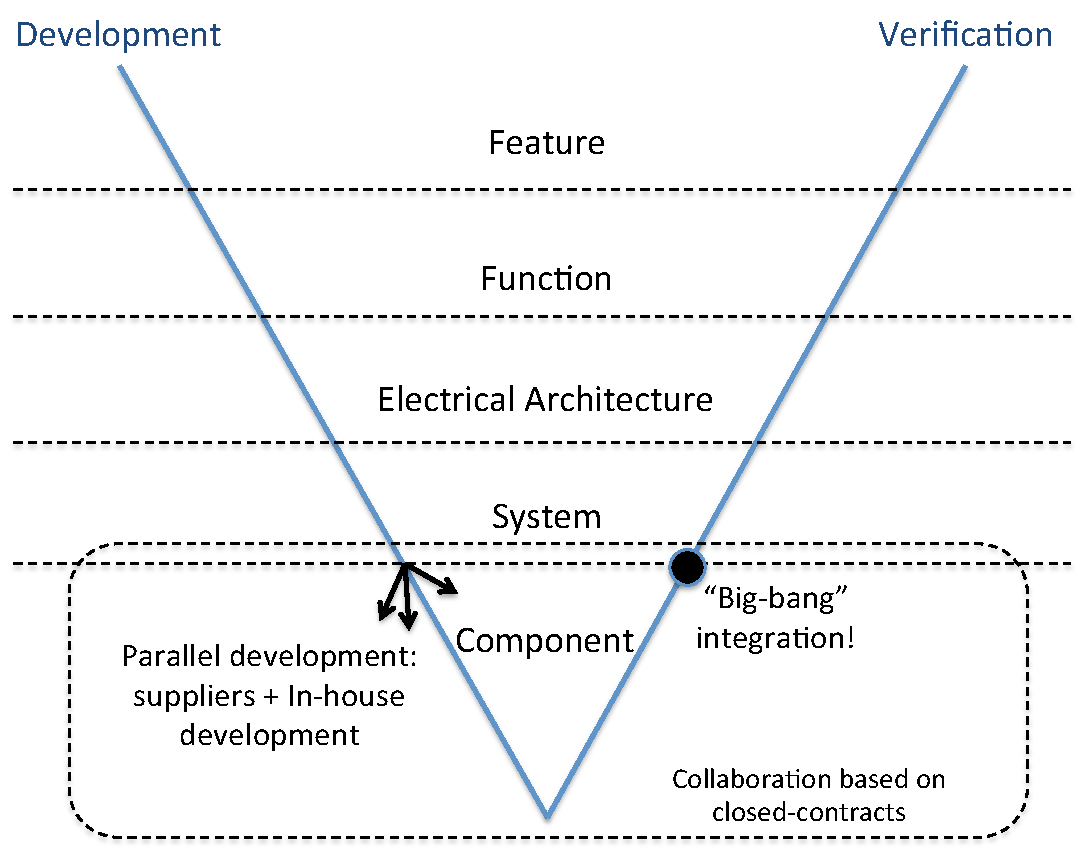
\includegraphics[width=\columnwidth]{figure/Closed-contract-collaboration.pdf}
\caption{Collaboration based on closed contracts}
\label{fig:closedContractCollaboration}
\end{figure}

Therefore, OEMs experience heavy reliance on external developers and subcontractors; this complicates coordination throughout the entire development process. Expensive communication and coordination delays during integration are results of outsourcing significant parts of development to suppliers. %This form of exponentially growing feature content severely complicates ``big-bang" integration~\cite{Eklund2012}. The development is inevitably parallelized; this obviously also holds for the large amount of externally developed software, which is integrated as black-box functionality~\cite{Patrizio2016AAF_Chalmers,Broy2009AAF_TUM,Broy:2006:CAS:1134285.1134292}. 

As shown in Figure~\ref{fig:closedContractCollaboration} the software engineering process follows the V-model, with the development on the left-hand side and verification on the right-hand side. The development at the level of components is parallelized among the different suppliers, and internal in-house development. The degree of parallelism can easily reach level 50 (i.e. 50 parallel developments). Once the collaboration between the OEM and its suppliers is regulated by closed-contract, the parallel developments represented in Figure~\ref{fig:closedContractCollaboration} start by signing a contract and then after months the large amount of externally developed software come back to the OEM and it is integrated as black-box functionality~\cite{Broy2009AAF_TUM,Broy:2006:CAS:1134285.1134292}. 
%the produced ECUs will be provided back to the OEM after some months with few communication during the production period.
This leads to the above mentioned ``big bang" integration~\cite{Eklund2012}. %: the developed Electronic Control Units (ECUs) (which include both hardware and software) come back to the OEM and integration starts. 
It is at this stage that many misunderstandings, conflicting interpretations, wrong assumptions, etc. are discovered.
It is easy to understand that closed-contract relations between the OEM and the suppliers can slow down the system-wide CI\&D.  %\todo{this last statement is disconnected from the rest of the story: miss the link between the mentioned integration problems and closed contracts}

%The collaboration between the stakeholders in the ecosystem needs to improve the software quality and provide faster, cheaper, and more predictable development~\cite{herbsleb2016IntelligentTransparent}. 
%
%This implies that the automotive (software) industry must identify how this new scenario\todo{what is the new scenario?} can be supported at best when an ecosystem of organizations collaborates.
%
%\todo{there is a gap between these two paragraphs: collaboration should be supported by new tools, like views and associated viewpoints to communicate the right architectural knowledge, etc.}
%
%These considerations motivate the need of considering new types of viewpoints and views\todo{add citation} from the perspective of specific system concerns, which are relevant for one or more stakeholders collaborating in the automotive ecosystem. Because of this, it is necessary for members of this ecosystem to agree on a common way of structuring\todo{what do you mean? structuring what?} in order to increase overall efficiency within the ecosystem \cite{Patrizio2016AAF_Chalmers,Broy2009AAF_TUM,Broy:2006:CAS:1134285.1134292}. An essential technical problem to solve for this vision is the establishment of standards for interoperability among IPs, both software and hardware, and tools \cite{Broy:2006:CAS:1134285.1134292}. ``Establishing and evolving ecosystems of different partner types might ultimately decide which companies win a market." \cite{Bosch2016Ecosystem}. First attempts, such as AUTOSAR \cite{acm2008autosar} and the Automotive Architecture Framework (AAF) \cite{Patrizio2016AAF_Chalmers,Broy2009AAF_TUM} are being developed. However, researchers and practitioners both identified the need for further research on this emerging type of software ecosystems.
%

\section{Research Method}\label{sec:researchMethod}

This section describes the research methodology and used in this work to address the research questions.
Our data collection was based on semi-structured interviews. 
The interview protocol follows the  seven-stage approach by Kvale \& Brinkmann~\cite{Kvale2015Interviews}. 
They suggest a process approach to conducting an interview. The seven-stage approach supports a consistent preparation, execution and reporting of the interview. This approach entails Thematising, Designing, Interviewing, Transcribing, Analysing, Verifying, and Reporting, as detailed in the following. The interviews provide in-depth analysis on the current situation and explore the desired situation. The results of the interview surveys are the foundation for the Reference Model\todo{What is that?}~\cite{Blessing:2009:DDR:1717807}. The goal of this section is to provide a clear description of the interview process applied in this research to support and clarify the results and present the results.

\subsection{Seven stages}

\noindent {\bf Thematising}: In this phase, the purpose and subject matter is defined, also, there are decisions made on the methods applied. The purpose of the interview surveys is to require in-depth information on the topics Continuous Integration \& Deployment and Ecosystem \& Transparency in the automotive industry. These topics are discussed with representatives of Volvo Car Corporation and its suppliers (Tier-1 and Tier-2). Also consultancy companies who work closely with the automotive industry are interviewed for this project.

\noindent {\bf Designing}: In this phase, the seven stages of the approach are designed. The structure of the interview survey, transcribing details, analysis protocol \cite{saldana2015coding}, verification and reporting are discussed in detail. Beforehand, the interviewee is informed on the interview details, topics and requested permission for the purpose of recording the conversation for the transcript. By doing this beforehand, the interviewee is familiar with the topics and allows him to prepare on the research topics. This is assumed beneficial for the results of the interview.

\noindent {\bf Interviewing}:  The interview is structured as a semi-structured interview. Instead of having specific questions for the whole interview, there were questions to guide the process and a list of goals that needed to be covered in the interview, so a discussion can arise. Semi-structured interviews are very suitable for exploratory research \cite{Runeson:2009:GCR:1519313.1519324}. The interview is divided in three categories: introduction, main questions and cool-off.
The introduction is meant to create context / background, and to provide and maintain an informal and interactive atmosphere. For the purpose of the research, it was necessary that the interviewee is able to explain as much as possible about their knowledge and experiences in their field of expertise in a short period of time. 
The main part of questionnaire is aimed at the actual research. The questions were meant to guide the interview, but it was necessary to be dynamic and interactive. This dynamic and interactive nature of interviewing is useful for exploration and development of interesting and unexpected ideas brought up by the interviewee, which could not have been possible with other (strict) methodologies, such as an interview questionnaire.
At the end of the interview or cool-off, the interviewee is given time to ask some questions about the topics, this could be topic or themes that are not mentioned in the interview or could be important for the research. Also an appointment is made with the interviewee to verify and validate the transcript.

\noindent {\bf Transcribing:} In order to be able to analyse the interview, it is required to transcribe the interview in a clear and precise manner. The interviewee and interviewer speak English and the interview will be held in English, hence, this is also the case for the transcript. Also the analysis or coding is done in English.

\noindent {\bf Analysing:} For the analysis of the interview, a protocol is applied to code the interview survey, retrieve useful information and analyse it for the research. This is done by the method explained by Saldana \cite{saldana2015coding}. The transcript is divided into smaller and easier to code parts. This could be words, phrases, sentences or sections. The goal of this analysis is to find keywords or themes that could be of value for the research. The findings are reported in the preliminary section of the coding table. This is done by constant comparison with the research, literature study and transcript in mind. After analysing the transcript and defining the preliminary codes, the final codes are defined based on relevance to the topics, importance, repetition or explicitly mentioned as important. The final codes are then used to make conclusions.

\noindent {\bf Verifying:} The activities in the verification phase include ascertaining the validity, reliability and generalizability of the findings. Validity refers to the question if the study investigates what was intended at the beginning \cite{Kvale2015Interviews}. The purpose of the interview is to obtain more insights and knowledge from the interviewee on the topics. The interview is semi-structured and the questions are intended as guidelines throughout the interview, so to safeguard validity. The guidelines are not meant to be strict, so it allows also to meander to address other related topics. By applying the systematic and structured approach by Kvale and Brinkmann \cite{Kvale2015Interviews}, the conducting, analysing and reporting of the interview process can be assumed as reliable. Hence, the results are considered reliable. The results of the research can be applied in more domains than the automotive industry, such as aviation. The most advanced cars have more or comparable software than (fighter) air planes\footnote{As said by Alfred Katzenbach, the director of information
technology management at Daimler: \url{http://spectrum.ieee.org/transportation/systems/this-car-runs-on-code}}. Moreover, we assume that the results are general applicable with similar contexts. 

\noindent {\bf Reporting:} The results of the analysis are reported in this thesis paper and will answer the research questions RQ1a and RQ1b) referred to in the introduction. These results will also support the Reference Model and this model will in return be the foundation of the (intended) Impact Model~\cite{Blessing:2009:DDR:1717807}. The Impact Model will be of advisory nature and will describe the desired, improved situation that is expected. These models are designed specifically for the domain of automotive software ecosystem, but by abstracting the models it is possible to apply them in other domains similar to the software ecosystem in the automotive industry, such as aviation.

\subsection{Analysis protocol}
For this research ten interview surveys were conducted with practitioners in a wide range of companies in the automotive software ecosystem. The interviews were transcribed and submitted in Atlas.ti \footnote{Qualitative Research tool Atlas.ti; https://atlasti.com}. This tool is used to manage quotations and codes of transcripts. The quotations and codes describe the train of thoughts of the interviewees in order to process them into feasible datasets and to help to support or negate propositions and research questions. All information that was relevant for the research was submitted as a quotation and connected to a code, including information that was not a direct answer to a research question or proposition. The codes were grouped into code groups to give an answer to one specific question, i.e. codes relevant to proposition 1 were submitted in code group "Proposition 1". This is done to simplify the writing process of the findings for each individual research questions and propositions. This entire process made it easy to group all relevant quotations in an overview and to create a selective dataset. This dataset was then further analysed to retrieve the answers on the questions of every interviewee. In addition, the dataset provide extra information that could benefit the findings for the specific question. This could be extra background information, another perspective on the question or maybe start a new discussion. The results of this process are the findings and answers to the research questions and propositions.
\section{Results}\label{sec:results}

In order to guide the
research and interview surveys %and to help the identification of the findings needed to answer the research questions 
we carefully formulated a set of propositions that will be then confirmed or negated by analysing the data collected through the semi-structured interviews we performed. Specifically, the first four propositions are defined for RQ1, propositions  5 and 6 are defined for RQ2,  and the remaining two are defined for RQ3.
The propositions aim at helping eliciting the different facets of transparency and contract-based collaborations and are based on knowledge that we acquired in numerous meetings we had with Volvo Cars and many suppliers within the NGEA and NGEA2 projects, and in our multi-annual and established collaboration with these companies. % and also on the result of literature review done
%prior to this research and are mapped as follows to the research questions: 

%\begin{table}[htb]
%\centering
%\begin{tabular}{|c|c|}\hline
%{\bf Research Question 1} & {\bf Research Question 2} \\ \hline % & {\bf Res. Quest. 4}\\ \hline
%		 &   \\ \hline
%		 & 	  \\ \hline
%		 &    \\ \hline
%		 &    \\ \hline
%		 & 	  \\ \hline		
%\end{tabular}
%\caption{Mapping propositions to research questions}
%\label{tab:mappingProRQs}
%\vspace{-.4cm}
%\end{table}


In Section~\ref{sec:ResearchQuestion1} we presents findings related to research question 1, in Section~\ref{sec:ResearchQuestion2} we presents findings related to research question 2,  in Section~\ref{sec:ResearchQuestion3} we presents findings related to research question 3, and finally
 in Section~\ref{sec:findings_RQs} we summarize the main findings and challenges.

\subsection{Research Question 1}\label{sec:ResearchQuestion1}

The propositions we defined for  
RQ1 (i.e. {\em What are the risks and/or benefits of increasing inter-organisational transparency?}) focus on these aspects:

\begin{itemize}
\item {\em Trasparency as necessary condition for  inter-organisational CI\&D}  - Proposition 1 %: Increasing inter-organisational transparency of information is a necessary condition for inter-organisational CI\&D
\item {\em Transparency is perceived positively/negatively within the companies} - Proposition 2 %: Increased inter-organisational transparency of information is considered positive
\item {\em It is easy to improve transparency} - Proposition 3 %: Inter-organisational sharing of information is considered simple between members of the projects
\item {\em There is a connection between transparency and quality of results of the project} - Proposition 4 %: A more open transparency policy improves the quality of the project and its results.
\end{itemize}

\vspace{.2cm}
\subsubsection{Proposition 1: Increasing inter-organisational transparency of information is a necessary condition for cross-organisational CI\&D}

This proposition states that information transparency across companies is necessary for inter-organisational CI\&D. The interviewees were asked how important inter-organisational transparency is for CI\&D and whether it is a necessity to pursue. 

During this research, we assumed inter-organisational transparency was a key factor for CI\&D processes across companies. However, the interview results {\bf reject the proposition}. Cross-organisational transparency has been identified as very important to pursue in general, but not a necessity for inter-organisational CI\&D. This answer to proposition 1 derives from the following findings:

\rog{if you ask the interviewees directly they will in general say that CI&D and transparency are two separate things, however, is this the case, look at this quotes below (can we really reject the proposition?). It might be that one can have successful project CI&D without transparency, but from the quote below, I read that it work even better with the combination. One of these quotes can be good to include as well?

Question: How important cross-organizational transparency on CI&D?

Quote: “I think it is very important, very important in general to increase efficiency. Very much for CI&D. These two are integrated as often as possible, then smaller issues will be erased on daily basis and another main concern is when an issue arise that we need to resolve quickly. I think when you need transparency, so we can take quick decision across organizations. Without transparency decision and discussion can take too long time.”


Here is another one I think relate to transparency:

Quote: “If you don’t have the transparency into the planning status. Then it would be very difficult for Volvo to know what they can expect. Even if you separate this, I still think that it is important for the recipient to know what they are about to get in to. If they don’t have this information beforehand, how can they plan their acceptance testing. “

Here is third one:

Quote: “if there is a problem in specifications, we will discuss this immediately. And if that change in specification does not really impact the amount of work, nor have any business impact then the specification will be updated.”

}

\noindent {\bf F1.1: Important, but not necessary.} The interviewees agree that the two topics together (information transparency and inter-organisational CI\&D) are indeed important, but not necessary. These two topics are integrated as often as possible, but also independent and successful as such, e.g. inter-organisational CI\&D without full transparency.

\noindent {\bf F1.2: Beneficial for synergy.} The interviewees agree that the combination of inter-organisational transparency and CI\&D produce synergy effects in terms of efficiency, trust, and mutual understanding.

\vspace{.2cm}
\subsubsection{Proposition 2: Increased inter-organisational transparency of information is considered positive}

Increasing inter-organisational transparency can be perceived differently by different stakeholders. The interviewees were asked how they considered the increase of transparency across companies, and how they perceived business and personal relationships between companies. The complexity of the project is experienced as an impediment working against full transparency of information.

However, the interview results {\bf support the proposition}, and the increase of information transparency is generally considered positive. This answer to proposition 2 is deduced from the following findings:

\rog{I like to be a little bit provocative. Yes, most of the interviews agreed, but I find the challenges with too much transparency very interesting:-

Question: Do you consider it is too much information?

Quote: “There is a lot of information and there is a risk with this amount of information. People will jump to conclusions when they see some bad numbers somewhere or something that is not happening … I would not say it is too much. It is more an issue of understanding how to use the information they get from us and we need to communicate in a different way”

Quote 2: “… it is difficult to manage to the new information. All of a sudden when you are completely transparent you also have to treat that information in a sensitive way.”

Quote 3: “I think sometimes the customer he may not want to know everything. I think some things you shouldn’t know as customer, because it might create unnecessary stress.”

Quote 4: “I think the dashboard is okay for this level of information, but if you go down one level maybe some technical issue the customers they shouldn’t need to know about. They will get fixed eventfully or other development situations.”

I like this one:

Quote 4: “When you go to a restaurant and you get your food, do you really need to know how dirty the kitchen is? If he food is okay, it is okay. It’s kind of that situation. When you start watching the chef and see if he washes his hands and you get into this where you start to wonder and worry about the chef and his qualities … Yes, I can reckon hat it can be too much information. Sometimes you don’t need to know what is happening in the kitchen.  For you own benefits and I know it sound terrible, but it is a conclusion I take sometimes you don’t need to know everything.” 

Quote 5: “One thing is Intellectual Property. You transfer knowledge and software between companies and it can be tricky license wise since we are building a Linus based platform which has many different source and components.”
}



\noindent {\bf F2.1: Increased transparency is positive.} All the interviewees experience positively the increase of inter-organisational transparency between companies and employees, for both business and personal relationships. The interviewees experience positive effects in terms of more awareness of the project status and increased mutual understanding. In particular, Volvo Cars employees found sharing a workplace with developers of the supplier especially effective for creating a shared mental model, thanks to the closer interaction with e.g. software developers.

\rog{supporting quotes 

Quote 1:  “ Normally, when we work with our customer we are not allowed to share our interval bug report details. But in this project, since we have our customer in our teams, they will see that kind of information.”
 
Quote 2: “ When we are doing our estimation or calculations of our prices, that is internally done. That is the setup today. It is a fixed price project, due to that. So we are still in a traditional OEM and supplier role”

Quote 3: “But if you compare it to other agile project that we have performed, then we have had at least one where we had a shared site and we were at the customers site. That was also good, because it was easy for the communication. I would think that in this project it is even better because we are sitting next to each other and are mixed. In the earlier project we were actually divided. We were sitting at xxx and there was a special area that was for supplier, so we were sitting there. The other area was for xxx. Even if we were sitting next to each other, it was still a little bit longer because you needed to go to their area. Rut if you are already mixed together, then type are like our colleagues.”

Quote 4: “ I would say that we nearly have full transparency. I would say transparency always goes 2 ways. Volvo is also sharing with us at the same level and they still keep 5\% information for themselves such s business critical information (future plans for example). But they are getting more and more open on that as well”

}

\noindent {\bf F2.2: Trust is increased.} The increase of transparency of information increases trust, too, on two levels. Firstly, increased trust between stakeholders improves collaboration and communication. Secondly, the trust gained in past projects (thanks to increased transparency of information) is more easily adopted in future projects as well.

\rog{Is trust increased due to being in the same office or due to transparency. I think it is more due to being in the same office, but we need to look at the interview results. It might be a combination of permitting more transparency and being in the same office. I have not done that so far}

\noindent {\bf F2.3: Create an understanding.} In some cases, the customer does not want or need to know everything, because this might create unnecessary stress. It is more an issue of understanding. 
% A quote by an open source manager: "When you go to a restaurant, do you really need to know how dirty the kitchen is? If the food is okay, it's okay." 

\rog{Seems a bit empty:-, add something more or remove it?}

\vspace{.2cm}
\subsubsection{Proposition 3: Inter-organisational sharing of information is considered simple between members of the projects.}

This proposition challenges the interviewees to critically evaluate the level of difficulty to share information across companies. In particular, the interviewees were asked about the difficulty to share information and the role of physical distance. The pilot project we are investigating (collaboration between Volvo Cars and a supplier) is perceived as a complex project by both companies. Due to the complexity of this project, the project members experience that it is difficult to work against full transparency of information with other stakeholders. 

The findings {\bf partially support the proposition}. The tooling and cross-organisational transparency, i.e. reducing physical distance, benefit cross-organisational information sharing, hence, reducing the complexity of a project. However, the automotive industry experiences difficulties to share information, and manage responsibilities and IPR. This answer to proposition 3 is deduced from the following findings:

\noindent {\bf F3.1: Reducing physical distance is beneficial for efficiency.} The interviewees agreed that reducing the physical distance between project members is the ideal situation for information sharing, thanks to shorter feedback loops. The new way of working introduced in the pilot project further enables both developers and management staff to share information more efficiently, thanks to Volvo Cars employees work alongside with the supplier employees, hence, making it simpler to share. 
% \todo{does the last sentence mean that the problem of distance is solved? or can we add that: future smarter working solutions will probably help mitigating this problem?}

\rog{However, I love this quote (I think we should include it):

Question: do you think that reducing the physical distance between members of a project is positive or a possible impediment?

Quote: “ It is always better that you can sit alongside each other. But it is a bit of generation question also. There are a lot of useful tools today, for example, Skype or Lync when it works. It is fixable, the younger people, this is my reflection, many of them are used to this, due to online gaming and such, they have no troubles of making this work … It will be feasible and possible to work even though you are placed in different companies or countries. I don’t think that is a big issue in the future."

So as you indicate smarter working solutions will probably help mitigating this problem, however, the question if we will ever be able to create trust being in different places:-

}

\noindent {\bf F3.2: Tooling support information sharing.} The tooling used for sharing information between developers or management staff is also a crucial factor for efficient information sharing across, but also within, companies. The interviewees from the pilot project are positive about the tools and their supportive role in the project and agree that it reduces the complexity of the project.

\rog{
I do not agree with the case that tooling support information sharing. They can support information sharing, but can also be a hinder: -

For, example (this is also a great quote):

Quote: “Let’s say for example we are using proprietary technology. Are the Supplier or Volvo proprietary, so that means that one of the parties have to adjust to this technology. The other part is always going to be behind and have difficulty to understand how everything should work.”

Moreover, they have made a visualisation tool to share information. This should be discussed. Visualization tools are important. 

}

\noindent {\bf F3.3: Managing responsibilities and IPR.} The automotive software ecosystem is experiencing safety, legal and responsibility issues. Therefore, it is extremely difficult to manage responsibilities (responsibility split) and IPR, for hardware and software. This is seen as an impediment and/or challenge for system-wide CI\&D.

\vspace{.2cm}
\subsubsection{Proposition 4: A more open transparency policy improves the quality of the project and its results.}

\rog{We have two factors here: more open transparency policy and being in the same office. It hard from the interviews to see which one has the largest effect:- Both seems to give positive results. Them main problem is that the contract stops both activities and transparency. Here we have several quotes against fix-prices, however, I don't know if this kind of quotes fit here, such as:

Question: Do you feel that there are constrains imposed by the contract now the project is ongoing?

Quote: Yes, I would say that in this case Volvo wants to work in an agile manner. That requires also basically agile contact. This is not really the case, This is in many sense stopping some of the activities...."

}

This proposition is developed to investigate whether the quality of the project results benefit from a more open transparency policy across companies. In particular, the interviewees were asked about the effects of this policy on the project and its results.

The findings {\bf support this proposition}:  the quality of the project and its results improve thanks to a more open transparency policy across companies. This answer to proposition 4 is deduced from the following findings:

\noindent {\bf F4.1: Overall project quality is increased.} The interviewees were unanimous about the positive effects of increased transparency on the quality of the project and its results. The quality improvements are already visible in the early stage of the project and they are confident about the improvements in the long term. An open transparency policy is positive for quality control because of mutual understanding of the project status and as a consequence gain in efficiency. Thanks to customer involvement, supplier employees also experience a healthy pressure that leads them to a higher quality level.

\noindent {\bf F4.2: Short feedback loops benefit project quality.} The more open transparency policy allows project members to have shorter feedback loops and as a consequence work more efficient.

\subsection{Research Question 2}\label{sec:ResearchQuestion2}

The propositions we defined for  
RQ2 (i.e. {\em Is there a lack or overload of information that is exchanged across organizations?}) focus on these aspects:

\begin{itemize}
\item {\em There is lack of information vs amount of information is sufficient} - Proposition 5 %: Project members have sufficient information to perform their activities
\item {\em Overload of information is/is not a problem} - Proposition 6
\end{itemize}

\vspace{.2cm}
\subsubsection{Proposition 5: Project members have sufficient information to perform their activities.}

This proposition challenges the interviewees to critically evaluate information, sent and received, between project members. They were asked what kind of information is (not) shared, if they have sufficient information available to perform their activities, and how this compares to other projects. All technical information is shared between project members, this includes source code, project information, and time planning. Commercial information is not shared between project members. This information contains strategic decisions, estimations, and third party agreements. The increased transparency across companies results in much more information than traditional projects, but equal or a bit more than agile projects. Third party agreements are an impediment for full transparency, because of licensing and responsibility issues.

The findings {\bf partially support this proposition}. On one side project members have sufficient information available for their activities, on the other side they are missing a holistic project overview. This answer to proposition 5 is deduced from the following findings:

\noindent {\bf F5.1: Project members have sufficient information.} Both companies, Volvo Cars and the supplier, state that they have sufficient information available from both companies to perform their activities. 

\noindent {\bf F5.2: An holistic project overview is needed.} The interviewees expressed that they miss an overview of their contribution in the product and in the overall project. They further agree that understanding their contribution in an holistic picture could benefit all stakeholders, because the involvement can increase project efficiency and quality.

\vspace{.2cm}
\subsubsection{Proposition 6: Information overload (in terms of frequent exchange) is unlikely to be considered a problem, if the exchanged information is precise}

We assumed that information overload could occur because of increased transparency between companies. This proposition was developed to challenge project members on how they experience information sharing. The interviewees were asked what kind of information is (not) shared, if it is much more or less information than other projects, and if they experienced information overload. {\em Information precision} is information sharing where supply and demand of information correspond. {\em Information overload} is information sharing where the receiving organisation receives more information than absolutely necessary. All the interviewees argued that information overload was not seen as a problem or risk.

The interview results {\bf support the proposition}, and information overload is unlikely to be considered a problem. This answer to proposition 6 is deduced from the following findings:

\noindent {\bf F6.1: Understanding thanks to collaboration.} Thanks to clear collaboration there is a shared understanding of the information which should be supplied or demanded by a stakeholder. This naturally contributes to information precision.

\subsection{Research Question 3}\label{sec:ResearchQuestion3}

The propositions we defined for  
RQ3 (i.e. {\em Are closed-contracts an impediment for scaling agility across company boundaries, and 
are industry-wide standards and processes shared among organizations an enabler?}) focus on these aspects:

\begin{itemize}
\item {\em Strict contract-based collaboration can be seen as an impediment for inter-organisational CI\&D}  - Proposition 7 
\item {\em Effects of adopting industry-wide standards and processes in a cross-organisational setting} - Proposition 8 
\end{itemize}

\vspace{.2cm}
\subsubsection{Proposition 7: Strict contract-based collaboration is an impediment for inter-organisational Continuous Integration and Deployment}

This proposition challenges how practitioners experience a strict (or closed) contract in a inter-organisational setting where companies work together in software engineering projects using CI\&D. During the interview survey, the interviewees were asked about the role of the contract when looking at information sharing and inter-organisational CI\&D. During the research it became clear that information sharing is seen as a crucial factor for inter-organisational collaboration. A closed contract regulates traditional project setups where the customer defines a list of requirements and the supplier has to fulfil it within a given time frame and budget. The automotive industry is traditional and relatively closed. It however emerges that it is changing towards more open collaborations, %greater inter-organisational transparency, 
participation in open source projects, and becoming a software-intensive sector. While still ongoing, this transition is confirmed by all interviewed stakeholders, and could lead to a cultural change toward adopting more open or flexible contracts for inter-organisational CI\&D.

The interview results {\bf support the proposition}: a strict contract-based collaboration is an impediment for inter-organisational CI\&D. This answer to proposition 7 is deduced from the following findings:

%\begin{figure}[htb]
%\centering
%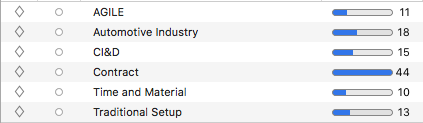
\includegraphics[width=\columnwidth]{figure/ss_CodeGroup6.png}
%\caption{Cultural change toward adopting more open or agile contracts for cross-organisational CI\&D}
%\label{fig:towardsAgile}
%\end{figure}

\noindent {\bf F7.1: Flexible contracts favour inter-organisational collaboration.} The interviewees share the opinion that a more open (or flexible) contract would be healthier for the project and benefit inter-organisational collaboration. Although some of the project members from both customer and supplier companies are not fully aware of the contract details, they do share the feeling of being restricted. They believe that strict contracts conflict with an agile way of working instead of supporting it, and suggest to adopt more flexible contracts, instead, also referred to as Time and Materials (T\&M) contracts\footnote{According to a T\&M contract, the contractor is being billed per hour regardless of the software project duration. If any additional features have to be developed the supplier charges just for the time spent by its employees working on a certain set of tasks [en.wikipedia.org]. This brings high flexibility to accommodate projects with evolving requirements, but also high uncertainty about the related costs.}. 
The interviewees agree that a T\&M contract allows for a better adaptation to project changes, distribution of resources, and it creates shared ownership otherwise hindered by closed contracts. They also argue in favour of a combination of a fixed price and T\&M contract, where stakeholders would agree on the product and cost estimation, but maintain high flexibility on how to produce it. This combination fulfils the need for flexibility and agility, but also the security for the customer. All interviewees made it clear that good collaboration between their companies is important from a legal and contractual perspective to support inter-organisational CI\&D.

% To preserve an open approach to the project, a product manager at a software development company suggests a combination of an agile and fixed price contract by creating project branches to avoid overhead in the main project.

\noindent {\bf F7.2: Closed contracts ease negotiation.} For a customer it is (still) more comfortable to work with closed contracts because one has more leverage and binds the supplier to pre-defined deliverables and deadlines. A Volvo Cars manager %involved in a RFQ projects, 
further states that it is hard for suppliers to negotiate with a T\&M or other flexible contracts, and that closed contracts make it easier competing with other suppliers.

% Accordingly, we elicit the following possible answers to proposition 6:

% \begin{itemize}
% \item Cross-organisational CI\&D benefits from a more open collaboration among companies, such as information sharing and adaptation to project changes. A strict contract is an impediment for this way of working related to cross-organisational CI\&D.
% \item A strict contract is an impediment for cross-organisational CI\&D. Although there is no direct connection between a strict contract and cross-organisational CI\&D, the way of working related to this method benefits from an open or agile contract.
% \item Cross-organisational CI\&D is possible with a strict contract, but synergy effects, i.e. collaboration and flexibility, are in effect when supported by an agile contract. By taking the synergy effects into account, a strict contract can be an impediment for Cross-Organisational CI\&D. An agile contract is difficult for a RFQ due to the open and uncertain characteristics of the contract.
% \end{itemize}

\vspace{.2cm}
\subsubsection{Proposition 8: Standards and processes, based on industry-wide data and process standards benefit cross-organisational CI\&D}

This proposition challenges the interviewees to experience the effects of industry-wide standards and processes in a inter-organisational setting where companies work together in software engineering projects using CI\&D. The interviewees were asked if they use industry-wise standards, and whether they find them beneficial for information sharing, which is important for cross-organisational CI\&D. The automotive industry is participating in various open source projects (e.g. AUTOSAR and GENIVI) and attempts to be good open source citizens. This development also enables companies to hire new employees easier, because open source knowledge is more common than knowledge of proprietary technology.

The interview results {\bf support the proposition}: industry standards and open source projects allow a common language and shared knowledge, therefore, benefits information sharing, which is important for inter-organisational CI\&D. This answer to proposition 8 is deduced from the following findings:

\noindent {\bf F8.1: Beneficial for information sharing.} The industry standards and open source projects allow a common language (i.e. AUTOSAR framework) and shared knowledge between project members; this improves communication and information sharing.

\noindent {\bf F8.2: Maturity and Management.} It is important for the success and adoption of open source projects and standards by stakeholder in the automotive industry, that these are highly controlled by one person, group or organisation. The maturity is also a crucial factor for the success or failure of an industry standard or open source project.



\subsection{Summary of the findings and challenges}\label{sec:findings_RQs}

In this section we summarize the findings and highlight the main challenges while giving an answer to the research questions.

\begin{itemize}
\item {\em RQ1: What are the risks and/or benefits of increasing inter-organisational transparency?} - Inter-organisational transparency is not a necessary condition for inter-organizational CI\&D. However, transparency is considered positive and creates positive synergy effects in terms of efficiency, trust, and mutual understanding while avoiding useless stressful situations. Transparency is also considered positive in terms of increasing the overall the project quality. 
There exist strategies to facilitate sharing inter organizations, however, the automotive industry experiences difficulties to share information, and manage responsibilities and IPR.
\item {\em RQ2: Is there a lack or overload of information that is exchanged across organizations?} - Increased transparency among organizations leads to much more information available to project members. In our pilot project participants feel that they have the information needed. However they are missing a holistic project overview. This ``big picture" could be beneficial for all stakeholders and can increase project efficiency and quality. Information overload in terms of frequency of updates is not considered a problem if the information exchanged is precise, i.e. supply and demand of information correspond.
\item {\em RQ3: Are closed-contracts an impediment for scaling agility across company boundaries, and 
are industry-wide standards and processes shared among organizations an enabler?} - Strict contract-based collaboration is an impediment for inter-organisational CI\&D. More flexible contracts will bring benefits to inter-organizational collaborations. However, closed-contracts facilitates negotiations between different organizations. Industry-wide standards and processes that are shared among organizations promotes collaborations, knowledge sharing, and communication. Open source initiatives help in the same direction and facilitate also the hiring process since people are already skilled. However, open source projects should be mature enough and the management of the project should be clearly controlled by a person, team, or organization.
\end{itemize}


The biggest challenges that steam out of our study are: 

\begin{itemize}
\item  {\em Challenge 1}: The automotive industry experiences difficulties to share information in the ecosystem, as well as to manage responsibilities and IPRs. 
\item {\em Challenge 2}: When the collaboration between different organizations is regulated though more ``open-contracts", it is not obvious  how to manage negotiations and responsibility sharing. It is also difficult to evaluate offers from different suppliers or from the supplier point of view, to compete transparently and well defined rules with other suppliers. 
\item {\em Challenge 3}: Means and strategies to share a ``big picture" of the project among the different stakeholders should be identified. A holistic view of the project could be beneficial for all stakeholders and can increase project efficiency and quality. 
\end{itemize}

%\pat{Add a summary and draw some conclusions}

%\begin{table}[htb]
%\centering
%\begin{tabular}{|c|c|c|c|}\hline
%{\bf Res. Quest. 1} & {\bf Res. Quest. 2} & {\bf Res. Quest. 3} & {\bf Res. Quest. 4}\\ \hline
%F3.3 & F2.1 & F3.1 & F9.1\\ \hline
%F6.2 & F2.2 & F3.2 & F9.2\\ \hline
%		 & F4.1 & F4.1 &\\ \hline
%		 & F4.2	& F6.2 &\\ \hline
%		 & F5.1 & F7.1 &\\ \hline
%		 & F6.1 & F8.1 &\\ \hline
%		 & 			& F8.2 &\\ \hline		
%\end{tabular}
%\caption{Mapping between research questions and findings}
%\label{tab:mapping}
%\vspace{-.4cm}
%\end{table}



% {\bf Industry Perspective.} 
% To preserve an open approach to the project, a product manager at a software development company suggests a combination of an agile and fixed price contract by creating project branches to avoid overhead in the main project.
%
%(Y)
% {\bf Maturity.} The automotive software ecosystem needs to adapt to the needs from the stakeholders. The industry is not mature enough, but is improving to adopt cross-organisational Continuous Integration and Deployment.
% Yes: Johnny Karlsson, Darrel Cullen, Lars Mattson, Petter Molder, Jacob Juul, Matti Larborn, 
% No: Anders Lindbom, Michael Svenstam, Mattias Almljum
\section{Discussion}\label{sec:discussion}

%\pat{How much upfront? What are the key artifacts that should be maintained?}
%\todo{I think this section should explain the implications of our results for SE.}
In this section we rely on Figure~\ref{fig:results} to discuss our findings. Where applicable, the discussion is organized from the perspective of industry (Section~\ref{sec:industry}) and academic research (Section~\ref{sec:research}).

Overall, we did not find a strong correlation between transparency and CI\&D, and in fact Proposition 1 has been rejected. However, in the specific of {\em inter-organizational} CI\&D, we found that increased information transparency (cf. left-hand side in the figure) %leads to having more information available among the project members that belong to different companies. Transparency
can have negative effects on privacy: by increasing transparency, organizations should be more aware of which information is sensitive and hence should or shouldn't share.
At the same time, transparency  positively influences project quality, trust, inter-organizational awareness and shared project understanding. This creates a good environment for inter-organizational CI\&D.

%\del{In this work we did not analyze functional safety assessment when CI\&D is involved. This is  interesting topic for future works; this topic would merit a dedicated study.}
Further, we found that when information transparency and inter-organizational CI\&D coexist, synergy (agile collaboration) increases, too. This confirms the potential benefits of applying agile development methodologies in ecosystems (like the automotive one) that target safety-critical systems and that are traditionally heavily controlled. In doing so, however, agile methodologies should remain conform to standards like the ISO 26262~\cite{iso26262} - a future challenge for both research and practice.
%\todo{Add discussion about functional safety assessment when CI\&D is involved. Check the works of Bruce Power Douglass, who pushes agile for ISO26262 for several years. He points out that the V model is more about relationships between work products and does not explicitly forbid the agile approach.}

%\del{In the following we discuss insights for practitioners (Section~\ref{sec:industry}) and a research agenda for researchers (Section~\ref{sec:research}).}

\subsection{Industry Perspective}\label{sec:industry}

This paper presented a pilot project of \company{} and one of its suppliers to investigate innovative ways of working and innovative collaboration models of the two organizations. 
Industries %\chg{that are thinking or that are already in the process of}{
interested in %} 
opening their platforms towards an ecosystem perspective, %\del{, or that simply are joining ecosystems} 
might benefit from our findings %\ins{
on adopting more agile and open collaborations. %}. \todo{I think these references to ecosystems could be removed. What about replacing it with companies that adopt more agile and open collaborations?}\eric{Love it, but considering the current status of our case study and the goals of NGEA, it could be nice to keep some small reference, if you do not think it hurts too much.}

%The proposition challenges interviewees to critically evaluate the impact of cross-organisational transparency on the business model strategy of their organisation. They were asked about the impact on the business model strategy on a functional and organisational level. 
%In general, the interviewees do not have an overview of the business model strategies of their organisation. 
%In addition to the findings already discussed above, in this section we want 
It is important to highlight that inter-orga\-ni\-za\-tional CI\&D could have an impact at both organizational and functional levels. 
%had a bigger impact in the early stage of the pilot project, but is getting less now the project is ongoing. 
%
%However, from our study it emerges that system-wide CI\&D %the interview results support the proposition, and cross-organisational transparency and CI\&D 
%could have an impact on business model strategies. %This answer to proposition 9 is deduced from the following findings:
%
%\noindent {\bf Impact on organisational level.} The organisational 
The {\em impact at an organisational level} is perceived differently by the two participating companies. For \company{}, it is perceived as one of the many projects and since they do not have the integration and end-responsibility for the product, it has not a big impact. However, for the supplier company, it is a high-risk experiment due to the complexity of the project. The employees of the supplier confirm that it has the highest complexity level the company accepted in its history.

%Th impact on functional level.} On functional level, 
The interviewees of both companies agree that the {\em impact at a functional level} of inter-organizational CI\&D %effects derived from the impact of cross-organisational transparency and CI\&D 
can be quantified in gain-in-efficiency, quality, and time-to-market. Also, CI\&D has less side effects than intermittent integration.%\del{, in case of big-bang integration.}  

For what concerns contracts, our findings suggest that traditional contracts are an impediment to inter-organizational CI\&D, but work well for what concerns negotiation and IPR. Innovative flexible contracts and/or ways of working are needed.

Finally, the interviewees state that, to date, inter-organizational CI\&D is not mature enough to predict the impact on collaboration models. 

\subsection{Academic Perspective}\label{sec:research}

%\todo{Improve the research agenda. It is introduced but not elaborated in details}

Researchers that are interested in scaling agile methodologies to the entire organization or to inter-organizational collaborations might find in this paper interesting findings coming from an industrial project in a challenging domain that is witnessing a profound transformation in the last years. 

%\todo{Below added the SE implications.}\\
Figure~\ref{fig:results} emphasizes (in dark-blue color) three aspects that we identified as the most relevant for software engineering researchers, along with the related indirect effects (in light-blue).
In particular, (1) to achieve the promised inter-organizational synergy, ecosystems need {\bf harmonized tooling} that can flexibility inter-operate to a.o. mitigate the (perception of) physical distance and implement (efficient) information sharing. Advances in service-oriented technologies, cloud integration and seamless software adaptation can provide the building blocks for such tooling. (2) As mentioned in the beginning of this section, further research is needed to  create effective {\bf information transparency}. Researchers working in software ecosystems can find in this paper an interesting example of ecosystem in the challenging automotive domain. Innovative ways to share information and knowledge within the ecosystem are needed. %We also considered only one OEM and one supplier. 
We also expect that different levels of sharing will be required within the same ecosystem, according to the degree of closeness of the OEM, to the level of trust, and to the purpose of the collaboration. Platforms are already being developed mostly addressing different levels of data sharing (e.g. KAVE~\footnote{\url{http://kave.io}}). Software engineering approaches are needed to define the sharing models and how to translate them into e.g. information generalization for controlled sharing. Further, approaches for information access should offer techniques to trace the individual contribution within the project shared in the ecosystem, and generate holistic project views for shared understanding. If present, these two techniques would help increasing project quality. Finally, our study highlighted how (3) the inter-organizational {\bf adoption of open-source software and standards} helps create a shared knowledge base and common language, which in turn further facilitate information sharing. Research in knowledge management applied to e.g. software architecture~\cite{akmbook} barely touched upon this topic.

% {\bf Industry Perspective.} 
%  To preserve an open approach to the project, a product manager at a software development company suggests a combination of an agile and fixed price contract by creating project branches to avoid overhead in the main project.
% 
%  {\bf Maturity.} The automotive software ecosystem needs to adapt to the needs from the stakeholders. The industry is not mature enough, but is improving to adopt cross-organisational Continuous Integration and Deployment.
% % Yes: Johnny Karlsson, Darrel Cullen, Lars Mattson, Petter Molder, Jacob Juul, Matti Larborn, 
% % No: Anders Lindbom, Michael Svenstam, Mattias Almljum

%\subsection{Open source}




%\rog{

%Discussion:
%
%One thing that surprised us analyzing the interviews, was the need for open source to obtain both more transparency and get CI\&D to run more smoothly. A Volvo employee said: ?I believe CI\&D is a model we must strive. I mean if you going to developing a very large system based on open standards. I think having this transparency should come natural, otherwise we will not. Volvo could order a Linux system and get this in a traditional way. We get binary report and get the delivery at the end and we could be happy. We will lose something, because we are building this software together and we have the rights to won and use them the future. Having Transparency and CI really gives a benefit to Volvo in the future reuse this assets, knowledge and experience.?. Another from Volvo is agree, but point out some problems as well, ?Yes. Open source is a very strong area related to CI as you say. Like you said, the tools are open source and the automotive industry is trying to keep this an open-source as possible. There are some week areas, like code coverage tools. They are very week, unfortunately, so we have to use commercial tools for that.?  Also the suppliers try to be as open as possible: ?? Some sources necessarily close. But we are trying to be as open as possible as requested.?.  It is also important to be active participation in the developing for open source: ?We are trying to be a good open source member by also upstreaming strategies, especially around GENIVI and Yocto. Here we find issues or improvements in the tools and we try to pass them back what we can. That is one of the strategies of the Supplier to work more open towards the open-source community as a give and receiver. We are working on that.? But, this might even be easier for Volvo: ?It is harder for the supplier. Since they in the end have to deliver the product on time and working after stream at least in the beginning it takes more time, because you need to align with the parties outside project. It might be a little bit problematic form them I think.?
%
%One of the strongest point is regarding knowledge of the tool, ?Let?s say for example we are using proprietary technology. Are the Supplier or Volvo proprietary, so that means that one of the parties have to adjust to this technology. The other part is always going to be behind and have difficulty to understand how everything should work.?
%
%}
\section{Related Works}\label{sec:relatedWorks}

\subsection{Continuous Integration and Deployment}

Continuous Integration (CI) is a development practice that assumes each developer to frequently commit their new code into a shared repository.
Every commit, triggers an automated build that verifies that the committed code is of sufficient quality by running various tests defined within the project. This enables faster feedback and allows the development team to detect problems early \cite{Fowler2006}.
By this, CI promises to improve release frequency and predictability, to increase developer productivity and communication \cite{Stahl2014}. 

While there is a relatively rich literature on how to implement and setup a small scale continuous integration for a project (e.g. \cite{Fowler2006,Neely2013}, there is lack of scientific support for how to scale such setups and also how to deal with involved hardware and complexities in embedded software \cite{Debbiche2014}. There are however works that report on challenges with scaling of continuous integration \cite{Roberts2004,Rogers2004} as well as with the applicability of agile approaches in the embedded domain \cite{Eklund2012a}.

Related to Continuous Integration are Continuous Delivery and Continous Deployment.
Continuous delivery is often referred to as ``a software development practice in which the software is kept in a state that, in principle, it could be always released to its users'' \cite{Humble2010}. 
In contrast, Continuous Deployment would require to not only deliver the software, but also to deploy it into the user's runtime.
Thus, Continuous Deployment becomes important when considering over the air updates to end-users.
Our paper, however, focuses on the continuous delivery between supplier and OEM, since we argue that this is the natural consequence of an OEM embracing system-wide continuous integration.

Rissanen and M\"unch \cite{Rissanen2015} addressed the challenges for companies in the domain of B2B making the transition towards continuous delivery and identified key aspects in technical, procedural and customer areas. While this study provide relevant insights it does not take into account the challenges involved in embedded and autonomous systems. 


\subsection{Ecosystem and Transparency}
Software ecosystems have been discussed from three distinct perspectives: Open source
\cite{Scacchi2009}, modelling and architecture (e.g. software evolution, architecture, and product lines \cite{Bosch2009}), and managerial perspectives (e.g. business aspects and co-innovation \cite{Jansen2012b}). 
Some degree of openness and transparency is a precondition for software ecosystems. Different degrees exist, from widely proprietary ecosystems to pure open source ecosystems \cite{Angeren2012,Jansen2012c}.
Jansen et al. \cite{Jansen2012a}, Bosch et al. \cite{Bosch2009}, and Manikas et al. \cite{Manikas2013b} discuss how to analyze software ecosystems and relationships among the actors of ecosystems. 
We consider the notion of a software ecosystem as a useful perspective on development work in the automotive software value-chain \cite{Knauss2014d} and by considering these related works, our study focuses on the specific interaction between automotive OEM and supplier.

One important aspect in our interviews has been the contract between both parties and the requirements defined there with respect to time and functionality. 
Not surprisingly, RE practice in traditional proprietary software projects (as e.g. described in \cite{Robertson1999,Ruhe2010}) differs significantly from the way requirements are handled in open source projects, where requirements are post-hoc assertions of functional capabilities and included into the system feature set after their implementation \cite{Scacchi2009}.
Knauss et al. indicate that requirements flows in open commercial ecosystems include a more open way of communicating requirements than in traditional approaches to Requirements Engineering (RE), while they the requirements processes and flows are different than in open source projects \cite{KYB+2016}. 


Transparency and emergent collaboration of stakeholders play a major role in driving requirements discussion and decision-making.
To our knowledge however, research has so far mainly investigated emergent developers \cite{Minto2007,Haenni2014,Sadi2015} and emergent knowledge \cite{Treude2012}, while only few and more recent works exist that start to investigate the effect of emergent contributors on requirements \cite{Kwan2011}, across organizations \cite{Linaker2016,KYB+2016}, and its implications with respect to transparency \cite{Dabbish2013,Hosseini2016}. 
We consider this an important research direction, since stakeholders with in-depth domain knowledge, the implicit knowledge about customer needs, their business domain and the system’s environment \cite{Damian2013}, must participate even when they span team or geographic boundaries \cite{boden2009bridging}.
In line with our findings, open communication channels have shown their value for building communities around healthy ecosystems  \cite{Kilamo2012}.
However, our results indicate that this transparency and information sharing needs to be carefully balanced: When planning transparency, one should specifically understand Stakeholders of information, as well as its usefulness, quality, and meaningfulness \cite{Hosseini2016}.
\section{Conclusion and Future Works}\label{sec:conclusion}

In this paper we investigated challenges and impediments of CI\&D that involves an OEM and one of its software suppliers.
This is a relevant topic since automotive OEMs have strong motivations to embrace CI\&D because of pressures of reducing the time to market and improving flexibility while keeping quality. Automotive OEMs are increasingly becoming software companies and most of the software is often produced by external companies, i.e. Tier-1 and Tier-2 suppliers, that populate the automotive ecosystem. 
For that reason, CI\&D in the automotive industry has to take into account also other actors of the ecosystem.  The increasing focus on software brings new challenges and opportunities for the software engineering field. 

More specifically, in this paper we investigated whether the way of working with suppliers should change while moving towards \ins{inter-organizational} CI\&D; then we focused on {\em contracts} that regulate the agreements between OEMs and suppliers, and   
%are mainly based on closed contracts.
on {\em transparency} that is intended as the degree/level of information that is shared among the organisations collaborating in the same value-chain. %within the ecosystem. 
The study has been performed within Volvo Cars in the context of a pilot and large project that is trying to reformulate the way of working within the ecosystem. Employees of the supplier company seat within Volvo Cars together with employees of the OEM and in some sense they work as a unique company, thus having more access to information. 
The results of the study show that more flexible contracts are needed, and that more transparency between OEM and suppliers is considered as an enabler for \chg{system-wide}{inter-organizational} CI\&D. 

As future work we plan to investigate the challenges found in this paper within other companies and possibly in domains that are different from the automotive one. Another future research direction is investigating whether the new way of working will trigger new business models within automotive domain, thus shifting towards a clearer and accepted win-win relationships between the actors of the ecosystem.

			

\balance

\bibliographystyle{IEEEtran}
\bibliography{bibliography}

\end{document}